\subsection{Skenario Pengujian}

\subsubsection{Load Testing}

Berikut adalah skenario yang digunakan untuk setiap varian pada load testing:

\begingroup
\footnotesize
\begin{longtable}{|l|l|l|l|}
    \caption{Skenario Load Test}                                                                    \\
    \hline
    \textbf{Skenario} & \textbf{Jumlah Iterasi} & \textbf{Banyaknya VUs} & \textbf{Durasi Maksimal} \\
    \hline
    \endfirsthead

    \multicolumn{4}{|l|}{\tablename\ \thetable\ -- \textit{Lanjutan dari halaman sebelumnya}}       \\
    \hline
    \textbf{Skenario} & \textbf{Jumlah Iterasi} & \textbf{Banyaknya VUs} & \textbf{Durasi Maksimal} \\
    \hline
    \endhead

    \hline
    \multicolumn{4}{|r|}{\textit{Dilanjutkan ke halaman berikutnya}}                                \\
    \endfoot

    \hline
    \endlastfoot

    sf-4              & 350.000                 & 10.000                 & 15 menit                 \\
    \hline
    sf-4              & 350.000                 & 12.000                 & 15 menit                 \\
    \hline
\end{longtable}
\endgroup

\subsubsection{Scaled-Down Simulation Test}

Berikut adalah skenario yang digunakan untuk Scaled-Down Simulation Test:

\begingroup
\footnotesize
\begin{longtable}{|l|l|l|l|}
    \caption{Skenario Scaled-Down Simulation Test}                                               \\
    \hline
    \textbf{Skenario} & \textbf{Jumlah Iterasi} & \textbf{VUs Puncak} & \textbf{Durasi Maksimal} \\
    \hline
    \endfirsthead

    \multicolumn{4}{|l|}{\tablename\ \thetable\ -- \textit{Lanjutan dari halaman sebelumnya}}    \\
    \hline
    \textbf{Skenario} & \textbf{Jumlah Iterasi} & \textbf{VUs Puncak} & \textbf{Durasi Maksimal} \\
    \hline
    \endhead

    \hline
    \multicolumn{4}{|r|}{\textit{Dilanjutkan ke halaman berikutnya}}                             \\
    \endfoot

    \hline
    \endlastfoot

    s10-2             & 40.000                  & 15.000              & 10 menit                 \\
    \hline
\end{longtable}
\endgroup

Arrival VUs ini mengikuti distribusi lognormal yang digambarkan pada grafik berikut:

\begin{figure}[htbp]
    \centering
    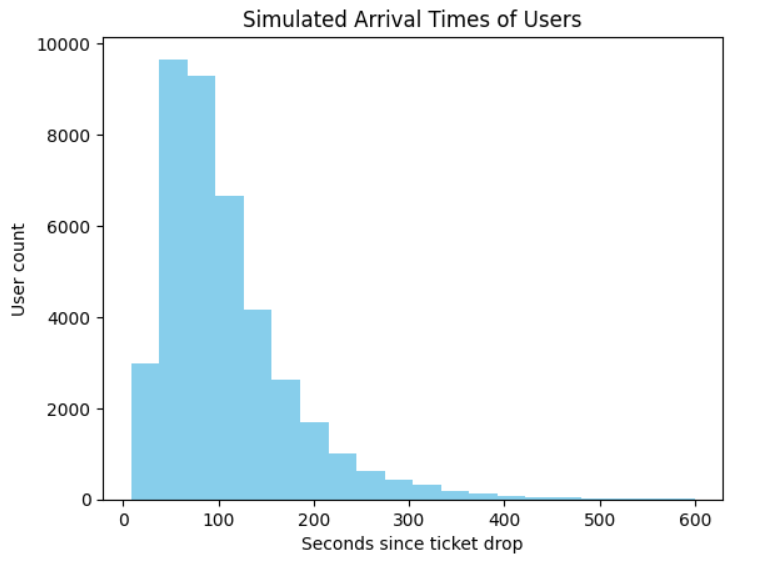
\includegraphics[width=1\textwidth]{resources/chapter-4/arrival-sim.png}
    \caption{Distribusi Arrival VUs}
    \label{fig:vus-arrival}
\end{figure}